\begin{enumerate}[label=\thechapter.\arabic*,ref=\thechapter.\theenumi]
\numberwithin{equation}{enumi}
\numberwithin{figure}{enumi}
\numberwithin{table}{enumi}

\item \begin{figure}[!ht]
    \centering
    \begin{circuitikz}
   \draw(0,0) to [R](2,0);
   % \draw (2,0) -- (2.5,0);
   \draw(2,0) to [L] (4,0);
   % \draw (5,0) to (5,0);
   \draw (4,0) to [C] (4,-2);
   \draw(4,-2)  to (0,-2);
   \draw (4,0) -- (5,0);
   \draw (4,-2)to (5,-2);
   \node[circle,fill,inner sep=1pt] at (0,0) {};
   \node[circle,fill,inner sep=1pt] at (5,0) {};
   \node[circle,fill,inner sep=1pt] at (5,-2) {};
   \node[circle,fill,inner sep=1pt] at (0,-2) {};
   \draw[->](0,-1.85) to (0,-0.15);
   \draw[->](5,-1.85) to (5,-0.15);
   \node at (0.3,-1) {$x(t)$};
   \node at (5.5,-1) {$y(t)$};

   \node at (1,0.5) {$R$};
   \node at (3,0.5) {$L$};
   \node at (2.8,-1) {$C$};\node[circle,fill,inner sep=1pt] at (0,0) {};
\end{circuitikz}

    \caption{RLC Low pass filter}
\end{figure}
\begin{table}[!ht]
    \centering
    \begin{tabular}{|c|c|}
\hline
    \textbf{Parameter} & \textbf{Description}  \\
    \hline
    $Z_C$ & Reactance of Capacitor \\
    \hline
    $Z_R$ & Reactance of Resistor \\
    \hline
    $Z_L$ & Recatance of Inductor \\
    \hline
    $x(t) = u(t)$ & Input Response \\
    \hline
    $y(t)$ & Output across capacitor \\
    \hline
    $\omega_0$ & Angular resonant frequency \\
    \hline
    \end{tabular}

    \caption{Input Parameters}
\end{table}
\begin{align}
    Y(s) &= I(s)Z_C\\
    &= \frac{X(s)}{Z_L + Z_R + Z_C}Z_C\\
    H(s) &= \frac{Y(s)}{X(s)}\\
    &= \frac{Z_C}{Z_L + Z_R + Z_C}\\
    &= \frac{\frac{1}{sC}}{sL + R + \frac{1}{sC}}\\
    &= \frac{1}{s^2LC + sRC + 1}\\
    \implies H(s) &= \omega_0^2\frac{1}{(s-p_1)(s-p_2)}
\end{align}
where,
\begin{align}
    \omega_0 &= \frac{1}{\sqrt{LC}}\\
    p_{1, 2} &= -\frac{R}{2L} \pm \sqrt{\brak{\frac{R}{2L}}^2 - \frac{1}{LC}}\\
    &= -\alpha \pm \sqrt{\alpha^2 - \omega_0^2}
\end{align}
where
\begin{align}
    \alpha &= \frac{R}{2L}
\end{align}
Damping Factor is given by,
\begin{align}
   \zeta &= \frac{\alpha}{\omega_0}\\
   &= \frac{R}{2}\sqrt{\frac{C}{L}}
\end{align}
\begin{table}[!ht]
    \centering
    \begin{tabular}{|c|c|c|c|}
\hline
    $\zeta$ & \textbf{Pole Location} & \textbf{Referred to as} & \textbf{Condition} \\
    \hline
    $\zeta > 1$ & Different locations on&&\\& the negative real axis & Overdamped & $R > 2\sqrt{\frac{L}{C}}$\\
    \hline
    $\zeta = 1$ & Coincide on&&\\& the negative real axis & Critically Damped & $R = 2\sqrt{\frac{L}{C}}$\\
    \hline
    $\zeta < 1$ & Complex Conjugate poles in&&\\& the left half of s-plane & Underdamped & $R < 2\sqrt{\frac{L}{C}}$\\
    \hline
\end{tabular}

    \caption{Effect of Damping Coefficient $\zeta$ on system behaviour}
\end{table}
\newpage
\begin{enumerate}
\item Overdamped Response
\begin{align}
    Y(s) &= X(s)H(s)\\
    &= \omega_0^2\frac{1}{s(s-p_1)(s-p_2)}\\
    &= \frac{c_0}{s} + \frac{c_1}{s-p_1} + \frac{c_2}{s-p_2}
\end{align}
where,
\begin{align}
    c_0 &= 1\\
    c_1 &= \frac{p_2}{p_1 - p_2}\\
    c_2 &= \frac{p_1}{p_2 - p_1}
\end{align}
Taking inverse Laplace,
\begin{align}
    y(t) &= c_0 + c_1e^{p_1t} + c_2e^{p_2t}\\
    &= \brak{1 + \frac{p_2}{p_1 - p_2}e^{p_1t} +  \frac{p_1}{p_2 - p_1}e^{p_2t}}u(t)
\end{align}

\begin{figure}[!ht]
    \centering
    \begin{tikzpicture}
      \draw[<->] (-4,0) -- (1,0) node[right] {$\mathcal{R}(s)$};
    \draw[<->] (0,-2) -- (0,2) node[above] {$\mathcal{I}(s)$};
  \draw[orange,thick] (-2.1,0.1) -- (-1.9,-0.1);
  \draw[orange,thick] (-2.1,-0.1) -- (-1.9,0.1);
  \draw[orange,thick] (-3.1,0.1) -- (-2.9,-0.1);
  \draw[orange,thick] (-3.1,-0.1) -- (-2.9,0.1);
  \node at (-3,-0.4) {\small $P_1$};
  \node at (-2,-0.4) {\small $P_2$};
\end{tikzpicture}

    \caption{s-Plane for Overdamped case}
\end{figure}

\item Critically Damped Response
\begin{align}
    Y(s)&=X(s)H(s)\\
    &= \omega_0^2\frac{1}{s(s-p)^2}\\
    &= \frac{c_0}{s}+\frac{c_1}{\left(s-p\right)^2}+\frac{c_2}{s-p}
\end{align}
where,
\begin{align}
    c_0 &= 1\\
    c_1 &= p\\
    c_2 &= -1
\end{align}
Taking Inverse Laplace,
\begin{align}
    y(t) &= c_0+(c_1t+c_2)e^{pt}\\
    &= \brak{1+(pt-1)e^{pt}}u(t)
\end{align}
\begin{figure}[!ht]
    \centering
    \begin{tikzpicture}
      \draw[<->] (-4,0) -- (1,0) node[right] {$\mathcal{R}(s)$};
    \draw[<->] (0,-2) -- (0,2) node[above] {$\mathcal{I}(s)$};
  \draw[orange,thick] (-2.1,0.1) -- (-1.9,-0.1);
  \draw[orange,thick] (-2.1,-0.1) -- (-1.9,0.1);
  % \node at (-3,-0.4) {\small $P_1$};
  \node at (-2,-0.4) {\small $p$};
\end{tikzpicture}

    \caption{s-Plane for Critically damped case}
\end{figure}

\item Underdamped Response
\begin{align}
    Y(s) &= X(s)H(s)\\
    &= \omega_0^2\frac{1}{s(s-p)(s-p^\ast)}\\
    &= \frac{c_0}{s}+\frac{c_1}{s-p}+\frac{c_2}{s-p^\ast}
\end{align}
where,
\begin{align}
    c_0 &= 1\\
    c_1 &= \frac{p^\ast}{p-p^\ast}\\
    c_2 &= \frac{p}{p^\ast-p}
\end{align}
Taking Inverse Laplace,
\begin{align}
    y(t) &= c_0+c_1e^{pt}+c_2e^{p^\ast t}\\
    &= 1+\frac{\abs{p}}{\omega_d}\ e^{-\sigma t}\frac{
    e^{j(\omega_d t+\varphi)}+e^{-j(\omega_d t+\varphi)}}{2}\\
    &= \brak{1+\frac{|p|}{\omega_d}e^{-\sigma t}\cos(\omega_d t+\varphi)}u(t)
\end{align}
where,
\begin{align}
    \abs{p}&=\sqrt{{\omega_d}^2+\sigma^2}\\
    \omega_d&=\omega_0\sqrt{1-\zeta^2}\\
    \sigma&=\omega_0\zeta\\
    \varphi&=\pi-\tan^{-1}\frac{\sigma}{\omega_d}
\end{align}
\begin{figure}[!ht]
    \centering
    \begin{tikzpicture}
    \draw[<->] (-4,0) -- (2,0) node[right] {$\mathcal{R}(s)$};
    \draw[<->] (0,-3) -- (0,3) node[above] {$\mathcal{I}(s)$};
       % \draw[blue, thick, ->] (-2,1) -- (0,2);
       %  \draw[blue, thick, ->] (-2,-1) -- (0,2);

  \draw [blue,arrows = {-Latex[width=0pt 10, length=10pt]}] (-2,1) -- (0,2);
   \draw [blue,arrows = {-Latex[width=0pt 10, length=10pt]}] (-2,-1) -- (0,2);

   \draw[brown, dashed] (-2,1) -- (0,1);
   \draw[brown, dashed] (-2,1) -- (-2,-1);
   \draw[brown, dashed] (-2,-1) -- (0,-1);
   \draw[red, dashed] (-2,1) -- (0,0);

   \node at (-2.2,1) {\small$P_{_1}$};
   \node at (-2.2,-1) {\small$P^*$};
   \node [orange]at (-1.7,0.2) {\small$-\sigma$};
   \node[blue] at (0.3,2) {\small $j\omega$};
    \node[brown] at (0.5,1) {\small $j\omega_d$};
    \node[brown] at (0.5,-1) {\small $-j\omega_d$};
    \node[red] at (-1.45,0.6){\small $\omega_0$};
    % \draw[dashed,->] (0,0.25) ++(-0.222:0.111) arc (90:153.5:0.25);
    \draw[brown,dashed,<->] (0,0.5) arc (90:153.5:0.5);
    \node [purple]at (-0.45,0.65) {\tiny$\sin^{-1}\zeta$};
\end{tikzpicture}

    \caption{s-Plane for Under damped case}
\end{figure}
\end{enumerate}
\begin{figure}
    \centering
    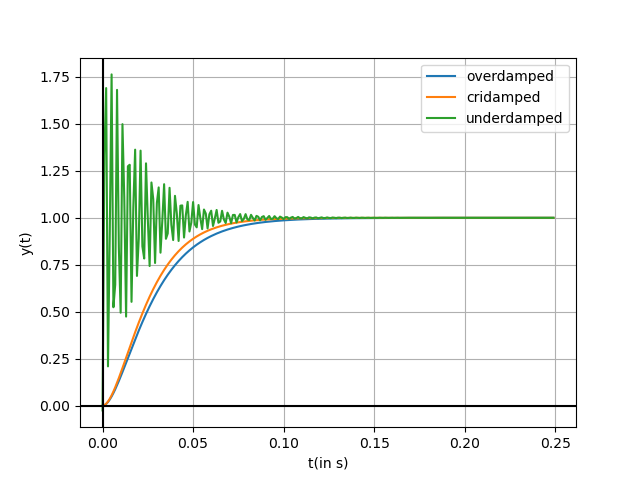
\includegraphics[width = \columnwidth]{app/figs/plot.png}
    \caption{Step response in all three cases}
\end{figure}

\end{enumerate}
